\subsection*{Zadania optymalizacyjne}
\subsubsection*{Zadanie~1.}
Oznaczmy przez \(w \in \open{0}{+\infty}\) szerokość tekstu na pojedynczej stronie (w~\(\cm\)). Skoro pole powierzchni zajętej przez tekst ma być równe \(150\cm^2\), to wysokość tekstu \(h\) musi wynosi \(\frac{150}{w}\). Do szerokości tekstu z~dwóch stron dokładamy po marginesie o~szerokości \(2\cm\), natomiast do wysokości z~góry i~z~dołu dokładamy po marginesie o~wysokości \(3\cm\). Zatem wymiary książki to
\begin{gather*}
    \pars{w + 2 \cdot 2} \times \pars{h + 2 \cdot 3}\\
    \pars{w + 4} \times \pars{h + 6}\\
    \pars{w + 4} \times \pars{\frac{150}{w} + 6}
\end{gather*}
Możemy zatem zdefiniować funkcję powierzchni pojedynczej strony w~zależności od szerokości tekstu \(w\):
\begin{equation*}
    S\pars{w}
        = \pars{w + 4}\pars{\frac{150}{w} + 6}
        = 150 + 6w + \frac{600}{w} + 24
        = 6w + 174 + \frac{600}{w} \qquad w \in \open{0}{+\infty}
\end{equation*}
Wyznaczmy pochodną tej funkcji:
\begin{equation*}
    S'\pars{w}
        = -\frac{600}{w^2} + 6
\end{equation*}
I~zbadajmy jej znak:
\begin{equation*}
    -\frac{600}{w^2} + 6
        = \frac{-600 + 6w^2}{w^2}
\end{equation*}
Mianownik jest dodatni, więc znak pochodnej zależy tylko od licznika:
\begin{equation*}
    -600 + 6w^2
        = 6\pars{w^2 - 100}
        = 6\pars{w + 10}\pars{w - 10}
\end{equation*}
Wykres znaku pochodnej:
\begin{equation*}
    \upparabola{-10}{10}[\(w\)]
\end{equation*}
Interesuje nas tylko przedział \(\open{0}{+\infty}\). Pochodna jest ujemna w~przedziale \(\open{0}{10}\), dla \(w = 10\) przyjmuje wartość \(0\), a~w~przedziale \(\open{10}{+\infty}\) jest dodatnia. Oznacza to, że funkcja \(S\) jest malejąca w~przedziale \(\open{0}{10}\) i~rosnąca w~przedziale \(\open{10}{+\infty}\), więc dla \(w = 10\) przyjmuje globalną wartość najmniejszą. Zatem optymalna szerokość pola tekstowego to \(10\cm\), a~jego wysokość to \(\frac{150\cm^2}{10\cm} = 15\cm\). Zatem wymiary książki to:
\begin{gather*}
    \pars{10 + 4} \times \pars{15 + 6}\\
    14 \times 21
\end{gather*}
Optymalna strona ma więc pole powierzchni równe \(294\cm^2\).
\subsubsection*{Zadanie~2.}
\begin{mathfigure*}
    \coordinate (A) at (3, 0);
    \coordinate (B) at (0, 4);
    \coordinate (C) at (0, 0);
    \coordinate (S) at (1.5, 2);
    \coordinate (M) at (2, 0);
    \coordinate (N) at (0, 8/3);
    \draw (A) node[below right]{\(A\)}
        -- (B) node[above left]{\(B\)}
        -- (C) node[below left]{\(C\)}
        -- cycle;
    \drawrightangle{A--C--B};
    \draw[ForestGreen] (M) -- (N) -- (S) -- cycle;
    \fillpoint*{M}[\(M\)][below];
    \fillpoint*{N}[\(N\)][left];
    \fillpoint*{S}[\(S\)][above right];
    \drawangle[RoyalBlue]{B--A--C};
    \drawangle[RoyalBlue]{N--M--C};
    \path (C) -- node[below]{\(x\)} (M);
\end{mathfigure*}
Zauważmy, że \(\mangle{NCM} = \mangle{BCA} = 90\degree\) i~\(\mangle{NMC} = \mangle{BAC}\). Zatem \(\triangle{NMC} \sim \triangle{BAC}\) w~skali \(\frac{x}{3}\), czyli
\begin{gather*}
    \frac{NM}{x} = \frac{BA}{CA}\\
    \frac{NM}{x} = \frac{5}{3}\\
    NM = \frac{5x}{3}
\end{gather*}
Pole \(\triangle{ABC}\) wynosi \(\frac{3 \cdot 4}{2} = 6\). Oznacza to, że jego wysokość opuszczona na bok \(AB\) ma długość \(\frac{2 \cdot 6}{AB} = \frac{12}{5}\). Zatem wysokość \(\triangle{NMC}\) opuszczona na bok \(NM\) wynosi \(\frac{x}{3} \cdot \frac{12}{5} = \frac{4x}{5}\). Wysokość \(\triangle{MNS}\) wyraża się zatem następująco:
\begin{equation*}
    h = \frac{12}{5} - \frac{4x}{5} = \frac{12 - 4x}{5}
\end{equation*}
Zdefiniujmy zatem funkcję pola \(\triangle{MNS}\) w~zależności od \(x\):
\begin{equation*}
    S\pars{x}
        = \frac{NM \cdot h}{2}
        = \frac{\frac{5x}{3} \cdot \frac{12 - 4x}{5}}{2}
        = \frac{60x - 20x^2}{30}
        = \frac{6x - 2x^2}{3} \qquad x \in \open{0}{3}
\end{equation*}
Wyznaczmy pochodną tej funkcji:
\begin{equation*}
    S'\pars{x}
        = \frac{1}{3}\pars{6 - 4x}
        = \frac{2}{3}\pars{3 - 2x}
\end{equation*}
Wykres znaku pochodnej:
\begin{equation*}
    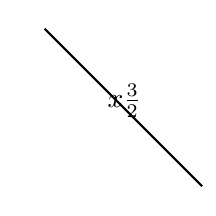
\begin{tikzpicture}
        \drawvec (-2, 0) -- (2, 0) node[below]{\(x\)};
        \draw[thick] (-1, 1) -- (1, -1);
        \fillpoint*{0, 0}[\(\frac{3}{2}\)][below left];
    \end{tikzpicture}
\end{equation*}
Interesuje nas tylko przedział \(\open{0}{3}\). Pochodna jest dodatnia w~przedziale \(\open{0}{\frac{3}{2}}\), dla \(x = \frac{3}{2}\) przyjmuje wartość \(0\), a~w~przedziale \(\open{\frac{3}{2}}{3}\) jest ujemna. Oznacza to, że funkcja \(S\) jest rosnąca w~przedziale \(\open{0}{\frac{3}{2}}\) i~malejąca w~przedziale \(\open{\frac{3}{2}}{3}\), więc dla \(x = \frac{3}{2} \in \open{0}{3}\) przyjmuje globalną wartość największą:
\begin{equation*}
    S\pars{\frac{3}{2}} = \frac{3}{2}
\end{equation*}
Zatem największe możliwe pole tego trójkąta jest przyjmowane dla \(x = \frac{3}{2}\) i~wynosi \(\frac{3}{2}\).
\subsubsection*{Zadanie~3.}
\begin{mathfigure*}
    \coordinate (A) at (0, 0);
    \coordinate (B) at (5.5, 0);
    \coordinate (C) at (5.5, 3);
    \coordinate (D) at (1.5, 5);
    \coordinate (E) at (0, 5);
    \coordinate (F) at (0, 4);
    \coordinate (G) at (3.5, 0);
    \coordinate (S) at (3.5, 4);
    \coordinate (Dprime) at (1.5, 0);
    \coordinate (Cprime) at (0, 3);
    \coordinate (X) at (1.5, 4);
    \coordinate (Y) at (3.5, 3);
    \coordinate (P) at (1.5, 3);
    \draw (A) node[below left]{\(A\)}
        -- node[below]{\(11\)} (B) node[below right]{\(B\)}
        -- node[right]{\(6\)} (C) node[above right]{\(C\)}
        -- (D) node[above right]{\(D\)}
        -- node[above]{\(3\)} (E) node[above left]{\(E\)}
        -- node[left]{\(10\)} cycle;
    \draw[dashed] (C) -- (Cprime) node[left]{\(C'\)};
    \draw[dashed] (D) -- (Dprime) node[below]{\(D'\)};
    \draw[ForestGreen] (F) -- (S) -- (G);
    \fillpoint*{S}[\(S\)][above right];
    \fillpoint*{X}[\(X\)][below left];
    \fillpoint*{Y}[\(Y\)][below right];
    \path (X) -- node[below]{\(x\)} (S);
    \path (Y) -- node[left]{\(y\)} (S);
    \drawrightangle[angle radius=0.4cm]{C--P--D};
    \drawrightangle[angle radius=0.4cm]{C--Y--S};
    \drawangle[angle radius=0.4cm, RoyalBlue]{D--C--P};
    \fillpoint*{P}[\(P\)][below left];
\end{mathfigure*}
Oznaczmy przez \(x\) długość odcinka \(XS\), a~przez \(y\) długość odcinka \(YS\). Zauważmy, że \(\mangle{CPD} = \mangle{CYS} = 90\degree\) i~\(\mangle{DCP} = \mangle{SCY}\). Zatem \(\triangle{SCY} \sim \triangle{DCP}\), czyli
\begin{gather*}
    \frac{SY}{YC} = \frac{DP}{PC}\\
    \frac{y}{8 - x} = \frac{4}{8}\\
    y = \frac{8 - x}{2}
\end{gather*}
Wymiary wycinanego prostokąta wynoszą \(\pars{x + 3} \times \pars{y + 6} = \pars{x + 3} \times \pars{\frac{8 - x}{2} + 6}\). Zdefiniujmy zatem funkcję pola powierzchni wycinanego prostokąta w~zależności od \(x\):
\begin{equation*}
    S\pars{x}
        = \pars{x + 3}\pars{\frac{8 - x}{2} + 6}
        = \frac{8x - x^2}{2} + 6x + \frac{24 - 3x}{2} + 24
        = \frac{17x - x^2 + 24}{2} + 24 \qquad x \in \closed{0}{8}
\end{equation*}
Wyznaczmy jej pochodną:
\begin{equation*}
    S'\pars{x}
        = \frac{1}{2}\pars{17 - 2x}
        = \frac{17}{2} - x
\end{equation*}
Wykres znaku pochodnej:
\begin{equation*}
    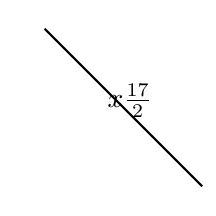
\begin{tikzpicture}
        \drawvec (-2, 0) -- (2, 0) node[below]{\(x\)};
        \draw[thick] (-1, 1) -- (1, -1);
        \fillpoint*{0, 0}[\(\frac{17}{2}\)][below left];
    \end{tikzpicture}
\end{equation*}
Interesuje nas tylko przedział \(\closed{0}{8}\). Pochodna jest dodatnia w~przedziale \(\open{0}{\frac{17}{2}}\), dla \(x = \frac{17}{2}\) przyjmuje wartość \(0\), a~w~przedziale \(\open{\frac{17}{2}}{+\infty}\) jest ujemna. Oznacza to, że funkcja \(S\) jest rosnąca w~przedziale \(\open{0}{\frac{17}{2}}\) i~malejąca w~przedziale \(\open{\frac{17}{2}}{+\infty}\), więc dla \(x = \frac{17}{2}\) osiąga globalną wartość największą, lecz \(\frac{17}{2} \not\in \closed{0}{8}\). Skoro maksimum nie leży w~dziedzinie, a~dziedzina jest domknięta, to ze względu na to, że funkcja jest rosnąca w~przedziale \(\open{0}{\frac{17}{2}}\), to wartość największą należącą do dziedziny funkcja osiąga na jej krawędzi:
\begin{equation*}
    S_\p{max} = S\pars{8} = 11 \cdot 6 = 66
\end{equation*}
Zatem optymalne wycięcie polega na odcięciu całego dolnego prostokąta \(11 \times 6\). Uzyskuje się wtedy kawałek o~polu powierzchni równym \(66\).
\subsubsection*{Zadanie~4.}
\begin{mathfigure*}
    \coordinate (A) at (0, 0);
    \coordinate (B) at (6, 0);
    \coordinate (S) at (3, 0);
    \coordinate (X) at (5, 0);
    \draw (A) -- (B);
    \fillpoint*{A}[\(A\)][left];
    \fillpoint*{B}[\(B\)][right];
    \fillpoint*{S}[\(S\)][above];
    \fillpoint*{X}[\(X\)][above];
    \path (S) -- node[below]{\(x\)} (X);
\end{mathfigure*}
Zauważmy na początek, że jeżeli \(X \in \set{A, B, S}\), to jeden z~czynników w~iloczynie \(AX \cdot SX \cdot BX\) jest równy \(0\), zatem cały iloczyn jest równy \(0\). Zauważmy ponadto, że jeżeli \(X \not\in \set{A, B, S}\), to żaden z~czynników nie jest równy \(0\), wszystkie są natomiast dodatnie, zatem wartość iloczynu jest dodatnia. Oznacza to, że pokrycie punktu \(X\) z~którymś z~puntków \(A, B, S\) na pewno nie jest optymalne. Skoro \(S\) jest środkiem odcinka \(AB\), który ma długość \(6\), to \(AS = BS = \frac{6}{2} = 3\) Konfiguracja jest symetryczna, więc na początek dla uproszczenia załóżmy, że punkt \(AX > BX\), jak na rysunku. Widzimy, że iloczyn, o~którym mowa w~zadaniu, można wyrazić następująco:
\begin{equation*}
    AX \cdot SX \cdot BX
        = \pars{AS + x}\pars{BS - x}x
        = \pars{3 + x}\pars{3 - x}x
        = 9x - x^3
\end{equation*}
Zdefiniujmy zatem funkcję tego iloczynu w~zależności od \(x\):
\begin{equation*}
    P\pars{x} = 9x - x^3 \qquad x \in \open{0}{3}
\end{equation*}
i~wyznaczmy jej pochodną:
\begin{equation*}
    P'\pars{x}
        = 9 - 3x^2
        = 3\pars{3 - x^2}
        = 3\pars{\sqrt{3} + x}\pars{\sqrt{3} - x}
\end{equation*}
Szkic wykresu pochodnej wygląda następująco:
\begin{equation*}
    \downparabola{-\sqrt{3}}{\sqrt{3}}
\end{equation*}
Interesuje nas tylko przedział \(\open{0}{3}\). W~przedziale \(\open{0}{\sqrt{3}}\) pochodna jest dodatnia, dla \(x = \sqrt{3}\) przyjmuje wartość \(0\), a~w~przedziale \(\open{\sqrt{3}}{3}\) jest ujemna. Oznacza to, że funkcja \(P\) jest rosnąca w~przedziale \(\open{0}{\sqrt{3}}\) i~malejąca w~przedziale \(\open{\sqrt{3}}{3}\), więc dla \(x = \sqrt{3}\) przyjmuje globalną wartość największą. Sytuacja jest symetryczna, gdy \(AX < BX\), po prostu punkt \(X\) leży w~odległości \(\sqrt{3}\) od~punktu \(S\), ale po jego drugiej stronie. Zatem optymalne punkty \(X \in AB\) to takie punkty, że \(SX = \sqrt{3}\). Wartość iloczynu wynosi wtedy
\begin{equation*}
    P\pars{\sqrt{3}} = 9\sqrt{3} - \pars{\sqrt{3}}^3
        = 9\sqrt{3} - 3\sqrt{3}
        = 6\sqrt{3}
\end{equation*}
\subsubsection*{Zadanie~5.}
\begin{mathfigure*}
    \coordinate (X) at (0, 0);
    \coordinate (A) at (-2, -4);
    \coordinate (B) at (1, -1.5);
    \coordinate (C) at (2, 4);
    \coordinate (D) at (-2.5, 3.75);
    \drawangle*[ForestGreen]{A--X--B}[\(\alpha\)];
    \draw (A) -- (B) -- (C) -- (D) -- cycle;
    \draw (A) -- (C);
    \draw (B) -- (D);
    \fillpoint{X};
    \path (A) -- node[above, sloped]{\(x\)} (X);
    \path (B) -- node[above, sloped]{\(y\)} (X);
    \path (C) -- node[above, sloped]{\(z\)} (X);
    \path (D) -- node[above, sloped]{\(d - x - y - z\)} (X);
\end{mathfigure*}
\begin{equation*}
    \begin{split}
        S
            &= \frac{1}{2}xy\sin\alpha + \frac{1}{2}yz\sin\pars{\pi - \alpha} + \frac{1}{2}z\pars{d - x - y - z}\sin\alpha + \frac{1}{2}\pars{d - x - y - z}x\sin\pars{\pi - \alpha}\\
            &= \frac{1}{2}xy\sin\alpha + \frac{1}{2}yz\sin\alpha + \frac{1}{2}z\pars{d - x - y - z}\sin\alpha + \frac{1}{2}\pars{d - x - y - z}x\sin\alpha\\
            &= \frac{1}{2}\sin\alpha\pars{xy + yz + z\pars{d - x - y - z} + \pars{d - x - y - z}x}
    \end{split}
\end{equation*}
Zauważmy, że \(\sin\alpha\) dla \(\alpha \in \rightclosed{0}{\frac{\pi}{2}}\) maksymalizuje się, gdy \(\alpha = \frac{\pi}{2}\) --- wynosi wtedy \(1\). Oznacza to, że na pewno, aby zmaksymalizować pole czworokąta, opłaca się ustawić przekątne prostopadle do siebie. Oznaczmy wtedy przez \(f\) długość jednej z~jego przekątnych. Wtedy druga przekątna ma długość \(d - f\). Zdefiniujmy zatem funkcję pola czworokąta w~zależności od \(f\):
\begin{equation*}
    A\pars{f} = \frac{1}{2}f\pars{d - f} \qquad f \in \open{0}{d}
\end{equation*}
Zauważamy, że jest to funkcja kwadratowa o~miejscach zerowych \(f = 0\) i~\(f = d\):
\begin{equation*}
    \downparabola{0}{d}[\(f\)]
\end{equation*}
Współczynnik kierujący jest ujemny, więc funkcja przyjmuje wartość największą dla \(f = \frac{d}{2} \in \open{0}{d}\). Zatem zbiór największych pod względem wielkości pola czworokątów z~przekątnymi sumującymi się do \(d\) jest zbiorem deltoidów, których przekątne mają równe długości. Pole wynosi wtedy
\begin{equation*}
    A\pars{\frac{d}{2}}
        = \frac{1}{2}\pars{\frac{d}{2}}^2
        = \frac{d^2}{8}
\end{equation*}
